\documentclass[10pt]{beamer}

\usetheme[progressbar=frametitle, background=light]{metropolis}
\usepackage{appendixnumberbeamer}

\usepackage{booktabs}
\usepackage[scale=2]{ccicons}

\usepackage{pgfplots}
\usepgfplotslibrary{dateplot}

\usepackage{graphicx}
\usepackage{xspace}
\newcommand{\themename}{\textbf{\textsc{metropolis}}\xspace}

\graphicspath{ {images/} }

\title{Introduction to Reinforcement Learning}
\subtitle{A primer on the concepts and algorithms}
\date{March 2, 2017}
\author{Krishnan Srinivasan}
\institute{Yale University}
% \titlegraphic{\hfill
\includegraphics[height=1.5cm]{logo.pdf}}

\begin{document}

\maketitle

\begin{frame}{Table of contents}
  \setbeamertemplate{section in toc}[sections numbered]
  \tableofcontents[hideallsubsections]
\end{frame}

\section{Introduction}

\begin{frame}{Reinforcement Learning}

  Reinforcement learning's popularity has spiked as a result of AlphaGo,
  which used a combination of Deep RL, CNNs, and Monte Carlo Search to
  beat the world's best Go player, Lee Sedol. Since then, it has evolved
  to become an even better player after competing in online Go competitions.

\end{frame}

\begin{frame}{Reinforcement Learning: Definitions}

  \begin{itemize}
    \item \textbf{Reinforcement learning problem:} An \textbf{agent} must learn to choose actions that allow it to transition from state to state in an environment, in order to get more reward.
    \item \textbf{Agent:} A Go-playing/helicopter-flying/etc. program
    \item \textbf{Environment:} A set of states and transitions (modeled as an MDP)
    \item \textbf{Policy:} $\pi: \mathcal{S} \rightarrow \mathcal{A}$
    \item \textbf{Total Discounted Reward:} $$G_t = R_{t+1} + \gamma R_{t+2} + \ldots = \sum_{k=0}^{\infty} \gamma^k R_{t+k+1}$$
    \item \textbf{Value:}
    \begin{enumerate}
      \item action-value function ~ $q_\pi: \mathcal{S} \times \mathcal{A}
        \rightarrow \mathbb{R}$
      \item state-value function ~ $v_\pi: \mathcal{S} \rightarrow \mathbb{R}$
    \end{enumerate}
  \end{itemize}

\end{frame}

\begin{frame}{Deep Reinforcement Learning}

  The main goal of reinforcement learning is to learn some optimal state-value/
  action-value function and (as a consequence) an optimal policy.
  One of the key advancements in RL has been the use of neural networks
  as function approximators to evaluate states (first done by Tesauro in
  TD-Gammon).

\end{frame}

\begin{frame}{What is Deep Reinforcement Learning?}

  Using neural networks to approximate
  \begin{itemize}
    \item value functions
    \item policy functions
    \item dynamic models (predicting future states/rewards)
  \end{itemize}

\end{frame}

\begin{frame}{Helicopter Apprenticeship Learning}
    \textbf{Example of apprenticeship learning:} \url{https://www.youtube.com/watch?v=M-QUkgk3HyE}
\end{frame}

\section{Temporal Difference Learning}

\begin{frame}{Temporal Difference Learning}

  The basis of the Q-Learning algorithm comes from the concept of
  \textbf{Temporal Difference Learning}.

  \textbf{Types of policy learning strategies:}
  \begin{itemize}
    \item Off-policy Learning: Evaluate a target policy $\pi(a|s)$ to compute
    $v_\pi(s)$ or $q_\pi(s,a)$. Learning by observation (with a guiding
    target policy). Apprenticeship learning is an example of this.
    \item On-policy Learning: Learn policy $\pi$ from experience gained from
    sampling $\pi$.
  \end{itemize}

\end{frame}

\begin{frame}{Temporal Difference Learning}

  \textbf{TD Learning} is the act of updating the values of your states
  while enacting the policy, to have a lower variance estimate of the actual
  value of a state. This is an example of "online" learning. \\An alternative
  to TD learning is known as \textbf{MC Learning}, which requires waiting
  until the end of an episode (policy evaluation until the terminal state),
  before updating the value estimates.

\end{frame}

\begin{frame}{Temporal Difference Learning}

  Generic TD learning update Step:
  $$ v'(s_t) \leftarrow v(s_t) + \alpha[R_{t+1} + \gamma v(s_{t+1}) - v(s_t)] $$

\end{frame}

\section{SARSA and Q-Learning Algorithms}

\begin{frame}{SARSA}

  \textbf{SARSA} stands for State, Action, Reward, State, Action, and comes
  from the parameters used in the SARSA algorithm. Both SARSA and Q-Learning use
  a temporal-difference prediction, which updates the value of a current
  state using an estimate of the next state's value plus the reward
  at the next state.

\end{frame}

\begin{frame}{SARSA}

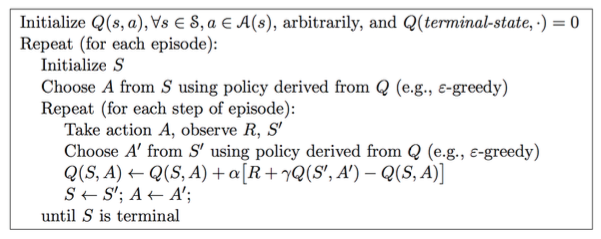
\includegraphics[width=\linewidth]{sarsa.png}

\end{frame}

\begin{frame}{Q-Learning}

  The algorithm for \textbf{Q-Learning} is almost identical to the SARSA
  algorithm shown in the previous slide, with the exception of the way the next state
  is chosen. In SARSA, the estimated value of a sampled state action pair
  for the next state is chosen to calculate the value of the current state.\\
  In Q-Learning, the next state always results from choosing the action
  that maximizes the $Q$ function, known as the action-value function. Q-Learning
  is an example of an off-policy approach towards learning the optimal
  action-value function. 

\end{frame}
  
\begin{frame}{Q-Learning}

    \begin{itemize}
        \item At each time step $t$, the action to change states is
            sampled from the current policy $A_{t+1} \sim \pi_t$.
        \item To measure the action-value of the current state-action
            pair $(S_t, A_t)$, the temporal difference update in Q-learning
            samples a different action $A'$ which is the action that
            maximizes the value of the next state $S_{t+1}$.
    \end{itemize}
    \begin{equation*}
        Q(S_t, A_t) & \leftarrow Q(S_t, A_t) + \alpha(R_{t+1} + \arg\max_{A'}\gamma Q(S_{t+1}, A') - Q(S_t, A_t))
    \end{equation*}

\end{frame}

\begin{frame}{Q-Learning}

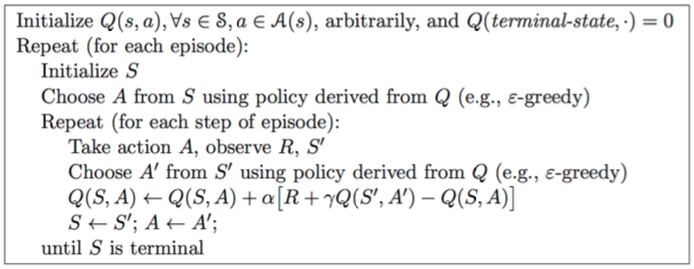
\includegraphics[width=\linewidth]{qlearning.png}

\end{frame}

\section{Code}

\begin{frame}{Code Tutorial}
    \begin{enumerate}
        \item Setup Python (install Homebrew if on MacOS)
        \item \href{http://jupyter.org/install.html}{\textbf{Juypter Notebooks}}
        \item \href{https://gym.openai.com/docs}{\textbf{OpenAI Gym}}
    \end{enumerate}
\end{frame}

\begin{frame}[standout]
  Questions?
\end{frame}

\appendix

\end{document}
